% $Id: introduction.tex 34630 2013-04-29 22:53:51Z roldeman $

\section{Optimising the $\alpha_T$ analysis for Run 2 data}
\label{sec:analysisOptimisation}

The major change with Run~2 of the LHC is the increase in energy to 13~TeV and instantaneous luminosity, to peak at $1.6\times10^{34}$~cm$^{-2}$s$^{-1}$, more than twice the peak of $7.7\times10^{33}$~cm$^{-2}$s$^{-1}$ reached in Run~1 \cite{LHCLuminosityIPAC13}. These two factors result in an increase in the number of simultaneous collisions per event and an increase in cross section for all SM processes. However, for SUSY particles outside the reach of Run~1 analyses, the relative increase in cross section increase should be greater than that for the backgrounds. It is therefore necessary to optimise the analysis to take account of the change in conditions. Some of the optimisations and alterations are discussed in this section.
\\\\
Events with a single hard jet and missing energy in their final state are particularly sensitive to the pair production of heavy invisible particles. They usually occur when the invisible system is produced in conjunction with initial or final state radiation from one of the colliding partons. To increase sensitivity to events with this topology, only the lead jet is required to have $p_T>100$~GeV, whereas in the Run~1 analysis this was required of the second leading jet. These extra results are added to an asymmetric jet bin, and have been seen to increase sensitivity to SUSY models with a compressed mass spectrum as well as generic models of dark matter pair production. The increase in yields for a compressed SUSY model by allowing a second jet with $p_T<100$~GeV is evident in Fig.~\ref{fig:asymMotivation}.
\\\\
\begin{figure}[h!]
  \centering
  \subfigure[Second jet $p_T$ for $200$~GeV$<H_T<250$~GeV, $\alpha_T>0.65$]{
    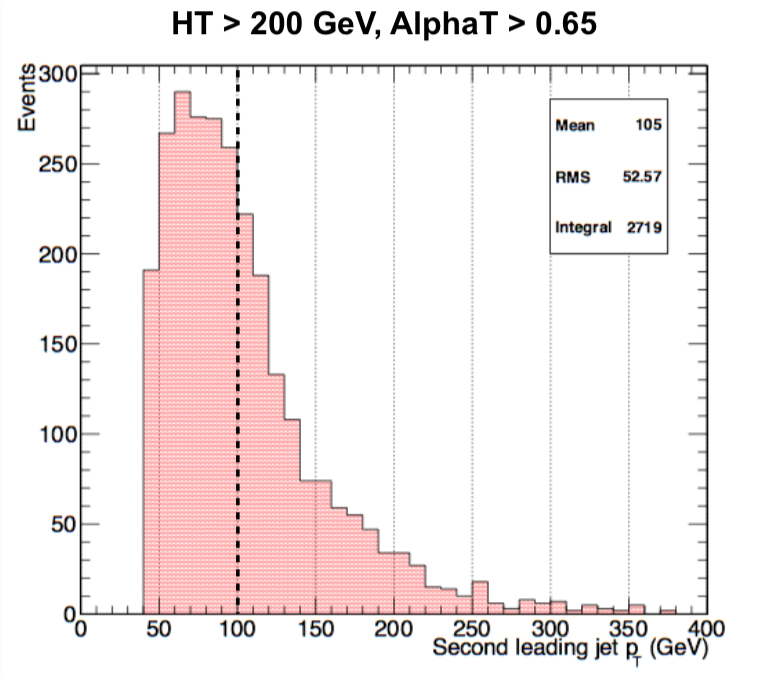
\includegraphics[width=0.5\textwidth]{secondJetPtlowHT}
  }~~
  \subfigure[Second jet $p_T$ for $400$~GeV$<H_T>500$~GeV, $\alpha_T>0.52$]{
    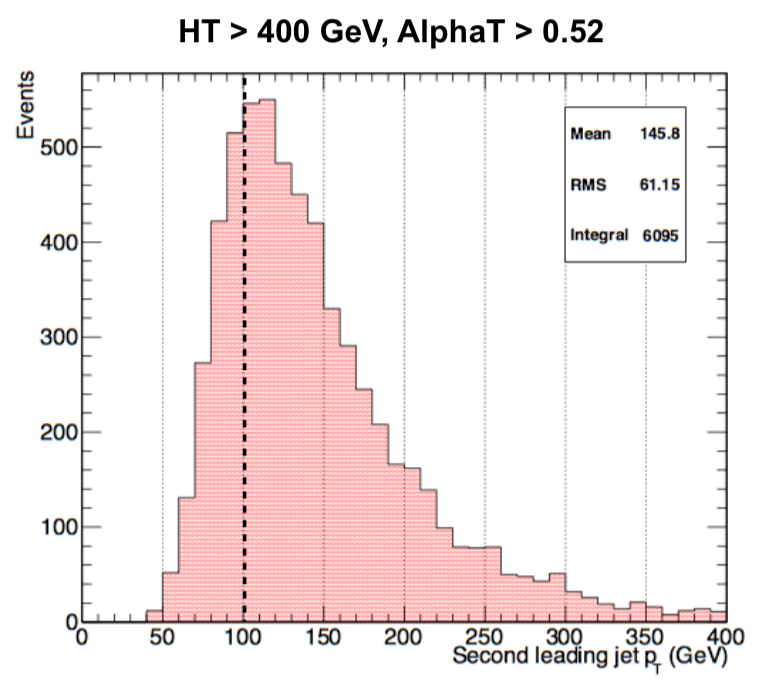
\includegraphics[width=0.5\textwidth]{secondJetPthigherHT}
  }
  \\
  \caption{\label{fig:asymMotivation} The second leading jet $p_T$ for different
  cases of $H_T$ after a baseline signal selection: $N_{jet}\geq2$, lead jet
  $E_T>100\gev$, lepton vetoes. Made with the T2tt ($m_{STOP}=425$~GeV, $m_{LSP}=325$~GeV) simplified model sample.}
\end{figure}

A significant alteration to the analysis is the decision to start categorising events by the amount of $\cancel{H_T}$ present
\\\\
One other particular study 